% Provenance (never printed): cycle 4 SVT/physique, "La planete Terre,
% l'environnement": uneven heating of the Earth, movements of the
% atmosphere, the global circulation and the climate zones; see
% sources/book1/PROVENANCE.md. Book 1, grade 8, chapter 2.
% Vocabulary guard: owns convection cell (atmospheric, descriptive), sea
% breeze and land breeze, the global winds, the global circulation. The
% Coriolis effect is told as "the Earth's rotation deflects"; Hadley and
% Ferrel cells and the intertropical convergence zone are named in prose
% only (Book 3 owns them); mantle convection is Book 2's.
\chapter{Angin dan Sirkulasi Global}\label{ch:g8:winds-global-circulation}

Selama berabad-abad, kapal-kapal layar yang meninggalkan pelabuhan-pelabuhan
Eropa dan Afrika menuju benua Amerika mengandalkan angin yang tetap dari
timur, yang bertiup di kedua sisi \omterm{def:g3:continents-and-oceans:equator}{khatulistiwa} dan membawa kapal-kapal itu
menyeberangi Atlantik. Para pelaut di seluruh dunia mengenalnya, dan
perdagangan awal dengan benua Amerika bergantung padanya: itulah
\emph{\omterm{def:g8:winds-global-circulation:global-winds}{angin pasat}}. Bahkan sekarang, kapal-kapal barang memanfaatkan \omterm{def:g8:winds-global-circulation:global-winds}{angin
pasat}, dan arus \omterm{def:g2:water-on-earth:ocean}{laut} yang digerakkannya, untuk mempersingkat pelayarannya.
% ledger: nos:trade-winds

\begin{omfigure}
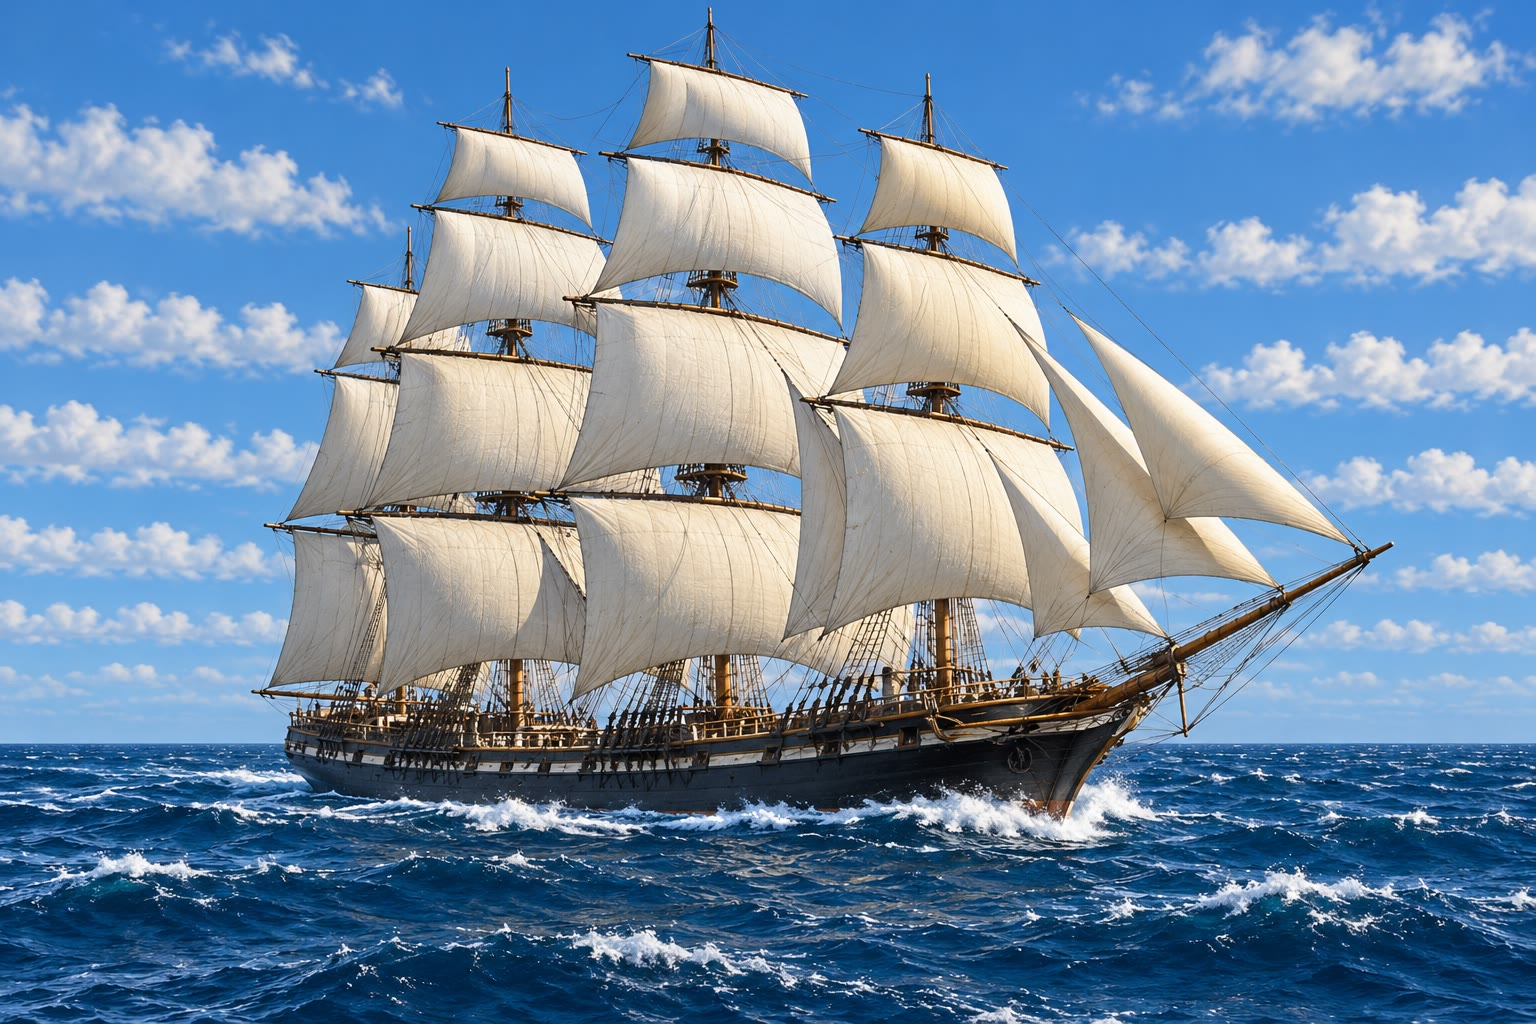
\includegraphics[width=0.62\linewidth]{images/book1/ai/g8-sailing-ship.jpg}

{\small Sebuah kapal layar yang melaju didorong angin yang tetap di \omterm{def:g2:water-on-earth:ocean}{samudra}
lepas (ilustrasi AI dari suatu adegan umum).}
\label{fig:g8:winds-global-circulation:ship}
\end{omfigure}

Mengapa \omterm{def:g8:winds-global-circulation:global-winds}{angin pasat} bertiup dari timur, dan selalu di tempat-tempat yang
sama? Mengapa ada \omterm{def:g5:weather-and-climate:desert}{gurun} di dekat \omterm{def:g5:weather-and-climate:tropics}{garis balik} dan \omterm{def:g5:weather-and-climate:rainforest}{hutan hujan} di dekat
\omterm{def:g3:continents-and-oceans:equator}{khatulistiwa}? Jawabannya dimulai dengan Matahari.

\begin{recall}
Angin adalah udara yang bergerak (buku-buku fisika). Udara menekan segala
sesuatu yang disentuhnya, dan tekanannya turun seiring \omterm{def:g4:world-physical-map:altitude}{ketinggian}
(\cref{ch:g8:the-atmosphere}). \omterm{def:g1:watching-the-weather:weather}{Cuaca} terjadi di \omterm{def:g8:the-atmosphere:layers}{troposfer}, lapisan
terbawah atmosfer. Bumi mempunyai \omterm{def:g5:weather-and-climate:climate-zone}{zona-zona iklim}: panas dan basah di
dekat \omterm{def:g3:continents-and-oceans:equator}{khatulistiwa}, dengan \omterm{def:g5:weather-and-climate:rainforest}{hutan hujan}; \omterm{def:g5:weather-and-climate:desert}{gurun} yang panas dan kering di
dekat \omterm{def:g5:weather-and-climate:tropics}{garis balik}; zona sedang, lalu zona dingin ke arah \omterm{def:g3:continents-and-oceans:poles}{kutub}
(\cref{ch:g5:weather-and-climate}).
\end{recall}

\section{Matahari memanaskan Bumi secara tidak merata}

Pada tengah hari pada hari ekuinoks, Matahari berada tepat di atas kepala
di \omterm{def:g3:continents-and-oceans:equator}{khatulistiwa}. Sinarnya tiba dengan curam di sana dan jatuh pada sepetak
kecil tanah. Lebih jauh ke utara atau ke selatan, sinar yang sama tiba
dengan miring dan tersebar pada petak yang lebih luas: setiap meter
persegi menerima lebih sedikit energinya. Pada \omterm{def:g6:latitude-longitude:latitude}{lintang} \ang{60}, berkas
yang sama menutupi tanah dua kali lebih luas daripada di \omterm{def:g3:continents-and-oceans:equator}{khatulistiwa},
sehingga setiap meter persegi mendapat separuhnya saja.
% ledger: (geometry: figdata/grade-8/sunlight_spread.py, spread = 1/cos(latitude))

\begin{omfigure}
\begin{tikzpicture}[font=\footnotesize]
  \def\R{2.6}\def\w{0.2}
  \fill[blue!10] (0,0) circle (\R);
  \draw (0,0) circle (\R);
  \draw[black!50] (-\R,0) -- (\R,0);
  \draw[black!40, dashed] (0,0) -- (60:\R);
  \draw[black!40] (0,0) ++(0:0.7) arc (0:60:0.7);
  \node at (25:0.95) {\ang{60}};
  \node[anchor=east, black!60] at (-\R-0.05,0) {khatulistiwa};
  % beam at the equator: rays between y = -w and y = w
  \foreach \y in {-0.2,-0.1,0,0.1,0.2} {
    \pgfmathsetmacro{\x}{sqrt(\R*\R-\y*\y)}
    \draw[orange!80!black, -{Stealth[length=1.6mm]}] (6.2,\y) -- (\x+0.03,\y);}
  \draw[omThm, line width=2.2pt] ({sqrt(\R*\R-0.35*0.35)},-0.35) arc ({asin(-\w/\R)}:{asin(\w/\R)}:\R);
  % beam near 60 degrees: rays between y = R sin 60 - w and + w
  \pgfmathsetmacro{\yc}{\R*sin(60)}
  \foreach \d in {-0.2,-0.1,0,0.1,0.2} {
    \pgfmathsetmacro{\y}{\yc+\d}
    \pgfmathsetmacro{\x}{sqrt(\R*\R-\y*\y)}
    \draw[orange!80!black, -{Stealth[length=1.6mm]}] (6.2,\y) -- (\x+0.03,\y);}
  \draw[omThm, line width=2.2pt] ({sqrt(\R*\R-(\yc-\w)^2)},\yc-\w) arc ({asin((\yc-\w)/\R)}:{asin((\yc+\w)/\R)}:\R);
  \node[anchor=west, align=left] at (6.3,0) {berkas yang sama\\pada petak yang kecil};
  \node[anchor=west, align=left] at (6.3,\yc) {berkas yang sama tersebar\\pada tanah dua kali lebih luas};
\end{tikzpicture}

{\small Dua berkas sinar Matahari yang identik pada tengah hari pada hari
ekuinoks. Di \omterm{def:g3:continents-and-oceans:equator}{khatulistiwa}, berkas itu jatuh tegak lurus pada petak yang
kecil (garis tebal); pada \omterm{def:g6:latitude-longitude:latitude}{lintang} \ang{60}, berkas itu miring dan menutupi
tanah dua kali lebih luas.}
% ledger: (geometry: figdata/grade-8/sunlight_spread.py)
\label{fig:g8:winds-global-circulation:beams}
\end{omfigure}

\begin{center}\small
\begin{tabular}{|l|c|c|c|c|c|}
\hline
\omterm{def:g6:latitude-longitude:latitude}{lintang} & \ang{0} & \ang{30} & \ang{45} & \ang{60} & \ang{75} \\
\hline
tanah yang ditutupi berkas yang sama & 1 & 1.15 & 1.41 & 2 & 3.86 \\
\hline
energi per meter persegi (\% dari \omterm{def:g3:continents-and-oceans:equator}{khatulistiwa}) & 100 & 87 & 71 & 50 & 26 \\
\hline
\end{tabular}
\end{center}
% ledger: (figdata/grade-8/sunlight_spread.py main table)

Selagi Bumi mengelilingi Matahari, sumbunya yang miring membuat Matahari
yang tepat di atas kepala bergeser di antara kedua \omterm{def:g5:weather-and-climate:tropics}{garis balik}, sehingga
terjadilah musim-musim (buku-buku fisika); tetapi sepanjang tahun,
wilayah-wilayah di dekat \omterm{def:g3:continents-and-oceans:equator}{khatulistiwa} menerima energi jauh lebih banyak
daripada wilayah-wilayah di dekat \omterm{def:g3:continents-and-oceans:poles}{kutub}. Pemanasan yang tidak merata ini
adalah penggerak utama angin: atmosfer membawa udara hangat ke arah \omterm{def:g3:continents-and-oceans:poles}{kutub}
dan udara dingin ke arah \omterm{def:g3:continents-and-oceans:equator}{khatulistiwa}.
% ledger: mo:global-circ

\section{Udara yang naik dan udara yang turun}

Udara hangat lebih ringan daripada udara dingin: udara hangat naik, dan
udara yang lebih sejuk di sekitarnya mengalir masuk untuk menggantikannya.
Di tempat udara naik, udara itu kurang menekan tanah: tekanan di sana
rendah. Di tempat udara turun, udara itu lebih menekan: tekanannya tinggi.
Di dekat tanah, angin bertiup dari tekanan tinggi ke tekanan rendah. Dengan
naik, mendingin, turun, dan mengalir kembali, udara itu berputar dalam
sebuah lingkaran.
% ledger: jetstream:sea-breeze, mo:three-cells

\begin{definition}[Sel konveksi]\label{def:g8:winds-global-circulation:convection-cell}
Yang disebut \emph{sel konveksi}\index{sel konveksi} di atmosfer adalah
lingkaran udara yang bergerak: udara yang dipanaskan dari bawah naik,
menyebar di \omterm{def:g4:world-physical-map:altitude}{ketinggian}, mendingin dan turun di tempat lain, lalu mengalir
kembali di sepanjang tanah ke tempat udara itu naik. Di bawah udara yang
naik, tekanannya rendah; di bawah udara yang turun, tekanannya tinggi.
\end{definition}
% ledger: jetstream:sea-breeze, mo:three-cells

\begin{inthelab}[Udara hangat naik]
Di dalam ruangan, guntinglah sebuah spiral dari selembar kertas tipis,
seperti kulit apel yang dikupas, lalu gantungkan spiral itu pada bagian
tengahnya dengan seutas benang. Peganglah spiral itu tinggi-tinggi di atas
radiator yang hangat pada musim dingin (jangan pernah di atas api atau
lilin): spiral itu perlahan-lahan mulai berputar. Udara yang dipanaskan
radiator naik dan mendorong spiral itu. Peganglah spiral itu di dekat
jendela yang dingin: apakah spiral itu berputar ke arah lain, atau tidak
berputar sama sekali?
\end{inthelab}

\omterm{def:g8:winds-global-circulation:convection-cell}{Sel konveksi} yang paling kecil dapat dirasakan pada hari yang cerah di
tepi pantai. Daratan dan \omterm{def:g2:water-on-earth:ocean}{laut} menerima sinar matahari yang sama, tetapi
sinar Matahari tidak masuk jauh ke dalam tanah, sedangkan \omterm{def:g2:water-on-earth:ocean}{laut} menyebarkan
panasnya ke lapisan air yang tebal. Jadi daratan menjadi jauh lebih panas
pada siang hari, dan jauh lebih dingin pada malam hari.
% ledger: jetstream:sea-breeze

\begin{omfigure}
\begin{tikzpicture}[font=\footnotesize, >={Stealth[length=2mm]}]
  \foreach \px/\title/\dir in {0/{Siang hari: angin laut}/1, 8.3/{Malam hari: angin darat}/-1} {
    \begin{scope}[xshift=\px cm]
      \fill[omSea] (0,0) rectangle (3.5,0.45);
      \fill[omLithAlluv] (3.5,0) -- (3.5,0.45) -- (7,0.75) -- (7,0) -- cycle;
      \draw (0,0.45) -- (3.5,0.45) -- (7,0.75);
      \node[anchor=south] at (3.5,3.25) {\textbf{\title}};
      \node at (1.75,0.22) {laut};
      \node at (5.6,0.3) {darat};
    \end{scope}}
  % day loop: surface sea -> land, rise over land, return aloft, sink over sea
  \draw[->, omDef, line width=1.1pt] (1.2,0.8) -- (5.2,0.95);
  \draw[->, omThm, line width=1.1pt] (5.8,1.1) -- (5.8,2.4);
  \draw[->, black!60, line width=1.1pt] (5.2,2.75) -- (1.2,2.75);
  \draw[->, omDef, line width=1.1pt] (0.6,2.4) -- (0.6,1.1);
  \node[omDef] at (3.2,1.25) {angin laut};
  \node at (0.6,0.75) {\textbf{T}};
  \node at (5.8,0.95) {\textbf{R}};
  \fill[yellow!80!orange] (6.6,2.7) circle (0.25);
  \node[anchor=north, align=center] at (1.75,-0.1) {laut lebih sejuk};
  \node[anchor=north, align=center] at (5.3,-0.1) {darat lebih hangat};
  % night loop: surface land -> sea, rise over sea, return aloft, sink over land
  \begin{scope}[xshift=8.3cm]
    \draw[->, omDef, line width=1.1pt] (5.2,1.0) -- (1.2,0.8);
    \draw[->, omThm, line width=1.1pt] (0.6,1.1) -- (0.6,2.4);
    \draw[->, black!60, line width=1.1pt] (1.2,2.75) -- (5.2,2.75);
    \draw[->, omDef, line width=1.1pt] (5.8,2.4) -- (5.8,1.15);
    \node[omDef] at (3.2,1.3) {angin darat};
    \node at (0.6,0.75) {\textbf{R}};
    \node at (5.8,1.0) {\textbf{T}};
    \fill[black!25] (6.6,2.7) circle (0.25); \fill[white] (6.72,2.78) circle (0.21);
    \node[anchor=north, align=center] at (1.75,-0.1) {laut lebih hangat};
    \node[anchor=north, align=center] at (5.3,-0.1) {darat lebih dingin};
  \end{scope}
\end{tikzpicture}

{\small \omterm{def:g8:winds-global-circulation:breezes}{Angin laut} dan \omterm{def:g8:winds-global-circulation:breezes}{angin darat}: dua \omterm{def:g8:winds-global-circulation:convection-cell}{sel konveksi} kecil yang berputar
dengan arah berlawanan. Panah merah: udara hangat yang naik; T dan R:
tekanan tinggi dan tekanan rendah di dekat tanah. Pada siang hari,
lingkaran itu mencapai \omterm{def:g4:world-physical-map:altitude}{ketinggian} 1000 sampai \qty{1500}{m}.}
% ledger: jetstream:sea-breeze
\label{fig:g8:winds-global-circulation:breezes}
\end{omfigure}

\begin{definition}[Angin laut dan angin darat]\label{def:g8:winds-global-circulation:breezes}
Yang disebut \emph{angin laut}\index{angin laut} adalah angin yang bertiup
dari \omterm{def:g2:water-on-earth:ocean}{laut} ke darat pada siang hari, ketika daratan lebih hangat daripada
\omterm{def:g2:water-on-earth:ocean}{laut}. Yang disebut \emph{angin darat}\index{angin darat} bertiup dari darat
ke \omterm{def:g2:water-on-earth:ocean}{laut} pada malam hari, ketika daratan sudah menjadi lebih dingin daripada
\omterm{def:g2:water-on-earth:ocean}{laut}.
\end{definition}
% ledger: jetstream:sea-breeze

\begin{omfigure}
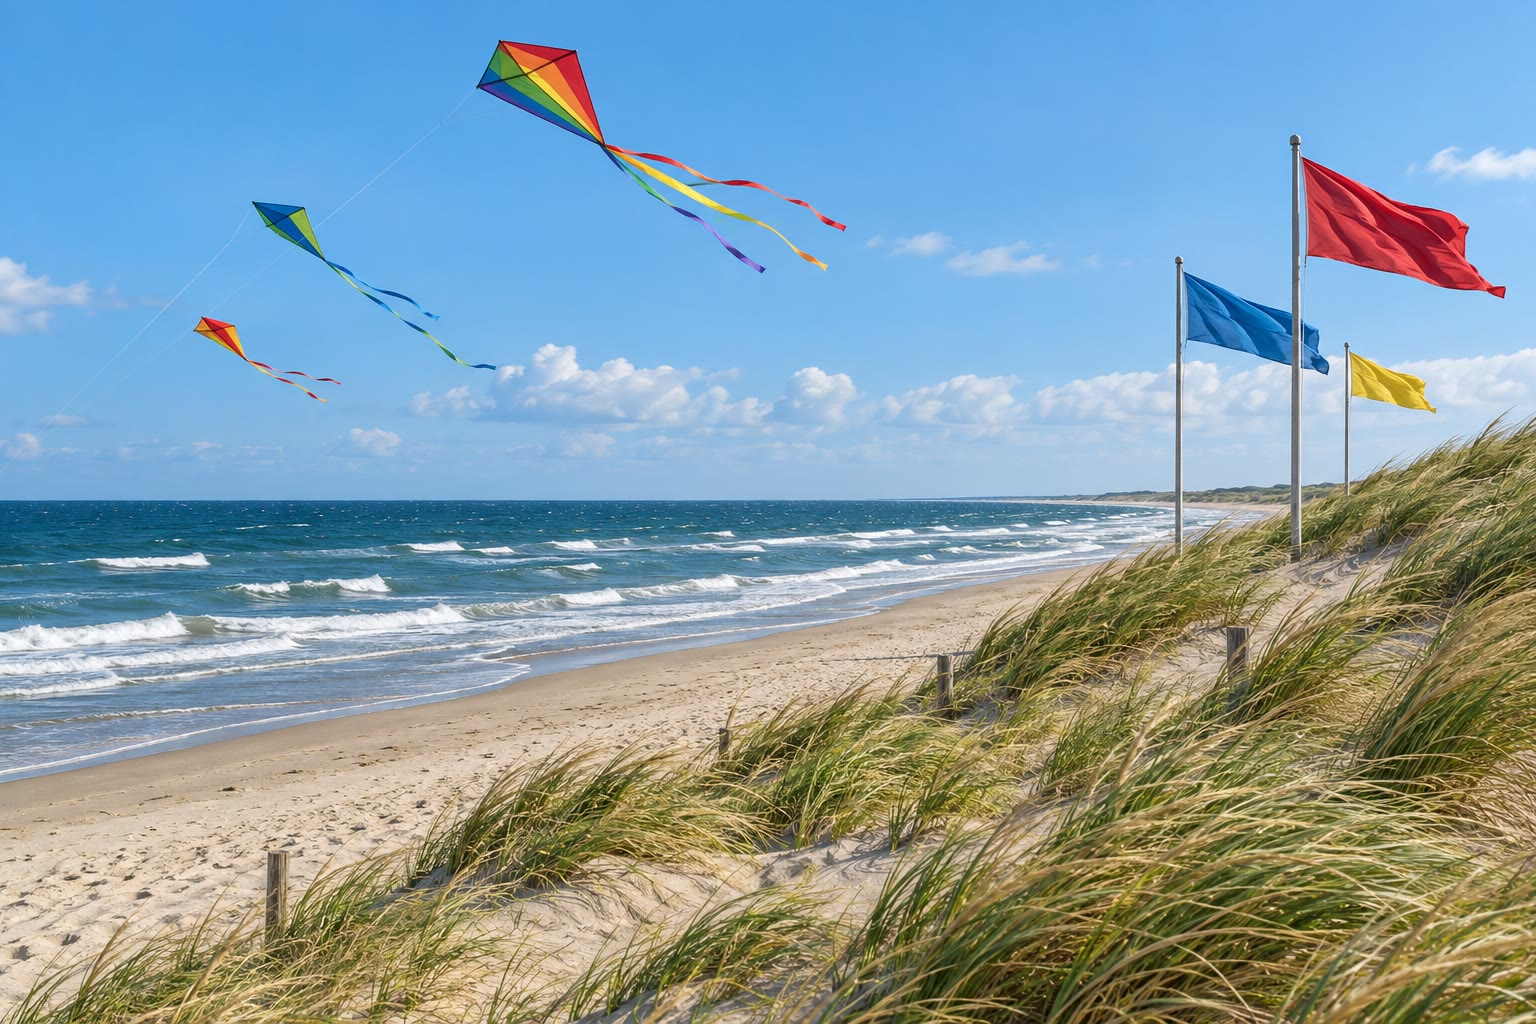
\includegraphics[width=0.55\linewidth]{images/book1/ai/g8-beach-kites.jpg}

{\small Layang-layang yang terbang dalam angin sore di sebuah pantai
(ilustrasi AI dari suatu adegan umum).}
\label{fig:g8:winds-global-circulation:kites}
\end{omfigure}

\section{Angin global}

Hal yang sama terjadi pada skala seluruh Bumi. Di dekat \omterm{def:g3:continents-and-oceans:equator}{khatulistiwa},
udara yang dipanaskan dengan kuat naik; udara itu menyebar ke arah \omterm{def:g3:continents-and-oceans:poles}{kutub} di
\omterm{def:g4:world-physical-map:altitude}{ketinggian} lalu turun lagi di dekat \omterm{def:g6:latitude-longitude:latitude}{lintang} \ang{30}. Jika dirata-ratakan
selama bertahun-tahun, \omterm{def:g8:the-atmosphere:layers}{troposfer} setiap \omterm{def:g3:continents-and-oceans:equator}{belahan bumi} berputar dalam tiga
\omterm{def:g8:winds-global-circulation:convection-cell}{sel konveksi} besar: satu dari \omterm{def:g3:continents-and-oceans:equator}{khatulistiwa} sampai kira-kira \ang{30}, satu
dari kira-kira \ang{30} sampai kira-kira \ang{60}, dan satu dari kira-kira
\ang{60} sampai ke \omterm{def:g3:continents-and-oceans:poles}{kutub}. Para ahli meteorologi menamainya sel Hadley, sel
Ferrel, dan sel \omterm{def:g3:continents-and-oceans:poles}{kutub}. Batas-batasnya bergeser mengikuti musim, dan sel
yang di tengah adalah rata-rata kasar dari banyak \omterm{def:g5:natural-hazards:storm}{badai} yang lewat.
% ledger: mo:three-cells, mo:global-circ, nos:doldrums

Angin yang bertiup di dekat tanah akan langsung bergerak dari tekanan
tinggi ke tekanan rendah seandainya Bumi tidak berputar. Karena Bumi
berotasi, udara yang bergerak dibelokkan: ke kanan di \omterm{def:g3:continents-and-oceans:equator}{belahan bumi utara},
ke kiri di \omterm{def:g3:continents-and-oceans:equator}{belahan bumi selatan}. Jadi udara yang mengalir kembali ke
\omterm{def:g3:continents-and-oceans:equator}{khatulistiwa} tidak datang dari utara, tetapi dari timur laut di \omterm{def:g3:continents-and-oceans:equator}{belahan
bumi utara} dan dari tenggara di \omterm{def:g3:continents-and-oceans:equator}{belahan bumi selatan}.
% ledger: mo:global-circ, nos:trade-winds

\begin{definition}[Angin global]\label{def:g8:winds-global-circulation:global-winds}
Angin di dekat permukaan yang paling sering bertiup di setiap sabuk \omterm{def:g6:latitude-longitude:latitude}{lintang}
adalah:
\begin{itemize}
  \item \emph{angin pasat}\index{angin pasat}, antara \omterm{def:g3:continents-and-oceans:equator}{khatulistiwa} dan
        kira-kira \ang{30}, yang bertiup dari timur laut di \omterm{def:g3:continents-and-oceans:equator}{belahan bumi
        utara} dan dari tenggara di \omterm{def:g3:continents-and-oceans:equator}{belahan bumi selatan};
  \item \emph{angin baratan}\index{angin baratan}, antara kira-kira \ang{30}
        dan \ang{60}, yang bertiup dari barat (dari barat daya di \omterm{def:g3:continents-and-oceans:equator}{belahan
        bumi utara}, dari barat laut di \omterm{def:g3:continents-and-oceans:equator}{belahan bumi selatan});
  \item \emph{angin timuran kutub}\index{angin timuran kutub}, antara
        kira-kira \ang{60} dan \omterm{def:g3:continents-and-oceans:poles}{kutub}, yang bertiup dari timur.
\end{itemize}
\end{definition}
% ledger: nos:trade-winds, mo:three-cells, mo:global-circ

\begin{omfigure}
\begin{tikzpicture}[font=\scriptsize, >={Stealth[length=1.8mm]}]
  \def\R{3}
  \fill[blue!8] (0,0) circle (\R);
  \draw (0,0) circle (\R);
  \draw[black!45] (-\R,0) -- (\R,0);
  \foreach \l in {-60,-30,30,60} {
    \pgfmathsetmacro{\y}{\R*sin(\l)}
    \pgfmathsetmacro{\x}{\R*cos(\l)}
    \draw[black!45, dashed] (-\x,\y) -- (\x,\y);}
  % surface winds: NE trades, SW westerlies, NE polar easterlies (north); mirrored south
  \foreach \x in {-1.8,-0.6,0.6,1.8} {
    \draw[->, omThm, line width=0.9pt] (\x+0.35,0.95) -- (\x-0.35,0.55);
    \draw[->, omThm, line width=0.9pt] (\x+0.35,-0.95) -- (\x-0.35,-0.55);}
  \foreach \x in {-1.2,0,1.2} {
    \draw[->, omDef, line width=0.9pt] (\x-0.35,1.7) -- (\x+0.35,2.02);
    \draw[->, omDef, line width=0.9pt] (\x-0.35,-1.7) -- (\x+0.35,-2.02);}
  \foreach \x in {-0.4,0.4} {
    \draw[->, omMeth, line width=0.9pt] (\x+0.25,2.85) -- (\x-0.25,2.65);
    \draw[->, omMeth, line width=0.9pt] (\x+0.25,-2.85) -- (\x-0.25,-2.65);}
  \node[fill=blue!8, inner sep=1pt] at (0,1.2) {angin pasat timur laut};
  \node[fill=blue!8, inner sep=1pt] at (0,-1.2) {angin pasat tenggara};
  \node[fill=blue!8, inner sep=1pt] at (0,2.3) {angin baratan};
  \node[fill=blue!8, inner sep=1pt] at (0,-2.3) {angin baratan};
  \node[anchor=south] at (0,\R+0.05) {angin timuran kutub};
  \node[anchor=north] at (0,-\R-0.05) {angin timuran kutub};
  % pressure belts on the left
  \foreach \l/\t in {90/{T: udara turun}, 60/{R: udara naik}, 30/{T: udara turun, kering, gurun}, 0/{R: udara naik, awan, hujan}, -30/{T: udara turun, kering, gurun}, -60/{R: udara naik}, -90/{T: udara turun}} {
    \pgfmathsetmacro{\y}{\R*sin(\l)}
    \pgfmathsetmacro{\x}{\R*cos(\l)}
    \draw[black!40] (-\x-0.05,\y) -- (-3.35,\y);
    \node[anchor=east] at (-3.4,\y) {\t};}
  \foreach \l/\t in {60/{\ang{60}\,LU}, 30/{\ang{30}\,LU}, 0/{khatulistiwa}, -30/{\ang{30}\,LS}, -60/{\ang{60}\,LS}} {
    \pgfmathsetmacro{\y}{\R*sin(\l)}
    \pgfmathsetmacro{\x}{\R*cos(\l)}
    \node[anchor=west, black!60] at (\x+0.05,\y) {\t};}
  % side view of the cells (height to the right), same latitude scale
  \begin{scope}[xshift=5.2cm]
    \draw[->] (0,-\R) -- (0,\R+0.3);
    \draw (0,-\R) -- (1.8,-\R);
    \node[anchor=north, align=center] at (0.9,-\R-0.05) {ketinggian di dalam\\troposfer $\rightarrow$};
    \foreach \lo/\hi/\cw in {0/30/0, 30/60/1, 60/90/0, -30/0/1, -60/-30/0, -90/-60/1} {
      \pgfmathsetmacro{\ya}{\R*sin(\lo)}
      \pgfmathsetmacro{\yb}{\R*sin(\hi)}
      \pgfmathsetmacro{\yc}{(\ya+\yb)/2}
      \pgfmathsetmacro{\bb}{max(0.09,(\yb-\ya)/2-0.06)}
      \ifnum\cw=0
        \draw[black!70, line width=0.7pt, postaction={decorate}, decoration={markings,
          mark=at position 0.125 with {\arrow{Stealth[length=1.6mm]}}, mark=at position 0.375 with {\arrow{Stealth[length=1.6mm]}},
          mark=at position 0.625 with {\arrow{Stealth[length=1.6mm]}}, mark=at position 0.875 with {\arrow{Stealth[length=1.6mm]}}}]
          (0.9,\yc) ++(0.75,0) arc (0:360:0.75 and \bb);
      \else
        \draw[black!70, line width=0.7pt, postaction={decorate}, decoration={markings,
          mark=at position 0.125 with {\arrow{Stealth[length=1.6mm]}}, mark=at position 0.375 with {\arrow{Stealth[length=1.6mm]}},
          mark=at position 0.625 with {\arrow{Stealth[length=1.6mm]}}, mark=at position 0.875 with {\arrow{Stealth[length=1.6mm]}}}]
          (0.9,\yc) ++(0.75,0) arc (360:0:0.75 and \bb);
      \fi}
  \end{scope}
\end{tikzpicture}

{\small \omterm{def:g8:winds-global-circulation:circulation}{Sirkulasi global}, disederhanakan. Kiri: sabuk-sabuk tekanan tinggi
(T) dan tekanan rendah (R) di dekat tanah. Pada bola bumi: angin di dekat
permukaan, yang dibelokkan oleh rotasi Bumi. Kanan: ketiga \omterm{def:g8:winds-global-circulation:convection-cell}{sel konveksi}
setiap \omterm{def:g3:continents-and-oceans:equator}{belahan bumi} dilihat dari samping, pada \omterm{def:g6:latitude-longitude:latitude}{lintang} yang sama (sel-sel
\omterm{def:g3:continents-and-oceans:poles}{kutub} digambar sangat tipis karena pita \omterm{def:g3:continents-and-oceans:poles}{kutub} sempit pada bola bumi).}
% ledger: mo:three-cells, mo:global-circ, nos:trade-winds, nos:doldrums
\label{fig:g8:winds-global-circulation:cells}
\end{omfigure}

\begin{method}[Menentukan angin global pada suatu lintang]\label{met:g8:winds-global-circulation:wind}
\begin{enumerate}
  \item Tentukan sabuknya: dari \omterm{def:g3:continents-and-oceans:equator}{khatulistiwa} sampai kira-kira \ang{30},
        dari \ang{30} sampai \ang{60}, atau dari \ang{60} sampai ke \omterm{def:g3:continents-and-oceans:poles}{kutub}.
  \item Tentukan ke arah mana udara mengalir di dekat tanah dalam sabuk
        itu: ke arah \omterm{def:g3:continents-and-oceans:equator}{khatulistiwa} pada sabuk pertama dan terakhir, ke arah
        \omterm{def:g3:continents-and-oceans:poles}{kutub} pada sabuk tengah.
  \item Belokkan aliran ini: ke kanan di \omterm{def:g3:continents-and-oceans:equator}{belahan bumi utara}, ke kiri di
        \omterm{def:g3:continents-and-oceans:equator}{belahan bumi selatan}.
  \item Sebutkan dari mana angin itu datang: angin dinamai menurut arah
        \emph{asal} tiupannya.
\end{enumerate}
\end{method}

\begin{example}[Angin pada lintang \ang{40}\,LS]\label{ex:g8:winds-global-circulation:40s}
Pada \ang{40}\,LS kita berada di sabuk tengah, antara \ang{30} dan
\ang{60}. Di sana udara di dekat tanah mengalir ke arah \omterm{def:g3:continents-and-oceans:poles}{kutub}, yaitu ke
arah selatan. Di \omterm{def:g3:continents-and-oceans:equator}{belahan bumi selatan}, udara itu dibelokkan ke kiri: bagi
udara yang bergerak ke selatan, kiri adalah timur, sehingga udara itu
akhirnya bergerak ke arah tenggara. Jadi udara itu datang dari barat laut:
itulah salah satu \omterm{def:g8:winds-global-circulation:global-winds}{angin baratan}, yang bertiup dari barat laut.
\end{example}
% ledger: mo:three-cells, mo:global-circ

Di dekat \omterm{def:g3:continents-and-oceans:equator}{khatulistiwa}, tempat \omterm{def:g8:winds-global-circulation:global-winds}{angin pasat} kedua \omterm{def:g3:continents-and-oceans:equator}{belahan bumi} bertemu,
angin mereda: para pelaut menyebut sabuk yang tenang ini
\emph{doldrum}. Udara yang hangat dan lembap naik di sana, mendingin, dan
menghasilkan \omterm{def:g4:clouds-rain-snow:precipitation}{hujan} deras dan badai petir yang terus-menerus. Di dekat
\ang{30}, di bawah udara yang turun, anginnya lemah dan \omterm{def:g4:clouds-rain-snow:precipitation}{hujan} jarang.
% ledger: nos:doldrums

\begin{definition}[Sirkulasi global atmosfer]\label{def:g8:winds-global-circulation:circulation}
Yang disebut \emph{sirkulasi global}\index{sirkulasi global} atmosfer adalah
gerakan udara berskala besar di sekeliling planet ini, yang terlihat jika
angin dirata-ratakan selama bertahun-tahun. Sirkulasi ini membawa panas dari
\omterm{def:g3:continents-and-oceans:equator}{khatulistiwa} ke arah \omterm{def:g3:continents-and-oceans:poles}{kutub}, dan uap air dari satu sabuk \omterm{def:g6:latitude-longitude:latitude}{lintang} ke sabuk
\omterm{def:g6:latitude-longitude:latitude}{lintang} yang lain.
\end{definition}
% ledger: mo:global-circ

\section{Sirkulasi global dan zona-zona iklim}

\omterm{def:g8:winds-global-circulation:circulation}{Sirkulasi global} menjelaskan sebagian besar \omterm{def:g2:drawing-to-map:map}{peta} \omterm{def:g5:weather-and-climate:climate}{iklim}. Di tempat udara
naik, di dekat \omterm{def:g3:continents-and-oceans:equator}{khatulistiwa}, udara itu mendingin dan uap airnya berubah
menjadi \omterm{def:g4:clouds-rain-snow:cloud}{awan}: \omterm{def:g4:clouds-rain-snow:precipitation}{hujan} sering turun, dan \omterm{def:g5:weather-and-climate:rainforest}{hutan hujan} tumbuh. Di tempat udara
turun, di dekat \ang{30}\,LU dan \ang{30}\,LS, udara itu menghangat selagi
turun, \omterm{def:g4:clouds-rain-snow:cloud}{awannya} mengering, dan \omterm{def:g4:clouds-rain-snow:precipitation}{hujan} jarang: \omterm{def:g5:weather-and-climate:desert}{gurun-gurun} panas yang besar,
seperti Sahara, terletak di sabuk-sabuk ini. Di \omterm{def:g6:latitude-longitude:latitude}{lintang} tengah, \omterm{def:g8:winds-global-circulation:global-winds}{angin
baratan} membawa \omterm{def:g5:natural-hazards:storm}{badai} demi \omterm{def:g5:natural-hazards:storm}{badai}, dengan \omterm{def:g4:clouds-rain-snow:precipitation}{hujan} pada semua musim.
% ledger: nos:doldrums, mo:three-cells, mo:global-circ

\begin{omfigure}
\begin{minipage}[c]{0.42\linewidth}\centering
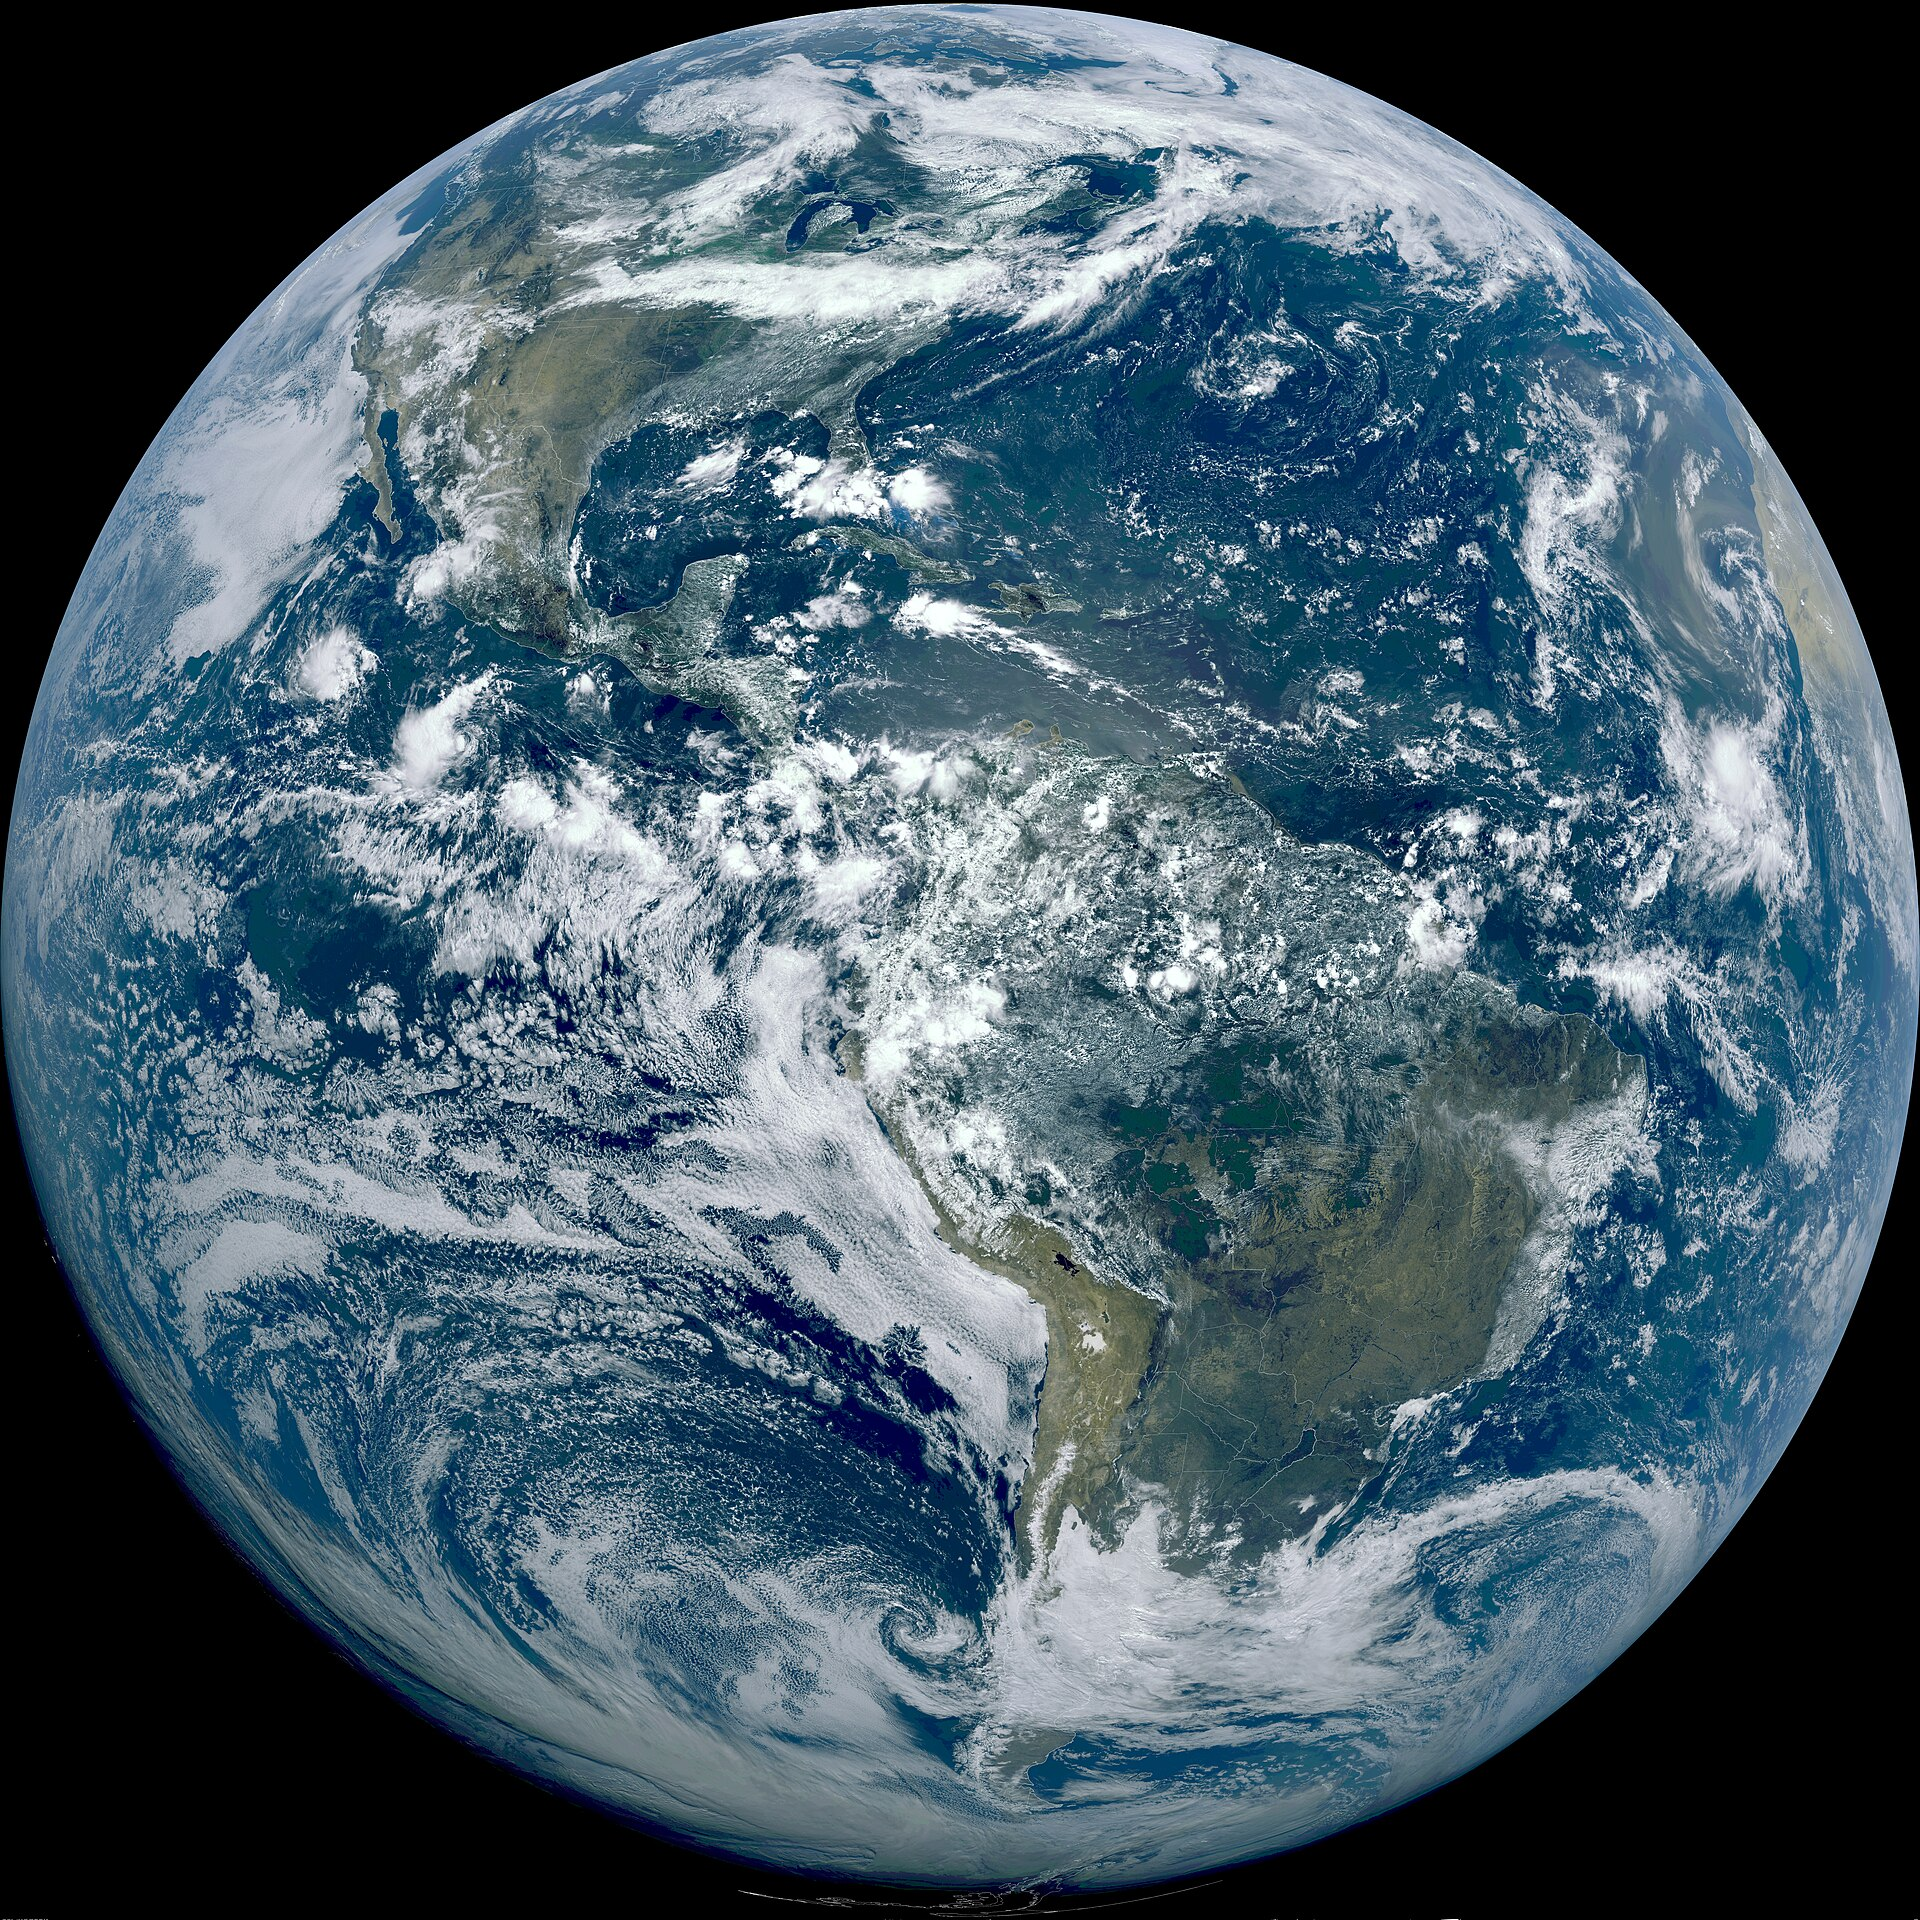
\includegraphics[width=\linewidth]{images/book1/g8-goes-full-disk.jpg}
\end{minipage}\hfill
\begin{minipage}[c]{0.54\linewidth}\raggedright
{\small Benua Amerika dilihat oleh satelit \omterm{def:g1:watching-the-weather:weather}{cuaca} GOES-16, tinggi di atas
\omterm{def:g3:continents-and-oceans:equator}{khatulistiwa}, pada tanggal 26~Juli 2022. Banyak \omterm{def:g4:clouds-rain-snow:cloud}{awan} telah terbentuk di
atas \omterm{def:g5:weather-and-climate:tropics}{daerah tropis} dan \omterm{def:g5:weather-and-climate:rainforest}{hutan hujan} Amazon, tempat udara yang hangat dan
lembap naik; jauh di selatan, pada musim dingin di \omterm{def:g3:continents-and-oceans:equator}{belahan bumi selatan},
\omterm{def:g5:natural-hazards:storm}{badai-badai} \omterm{def:g8:winds-global-circulation:global-winds}{angin baratan} berpusar di atas \omterm{def:g2:water-on-earth:ocean}{samudra}. NOAA (domain publik,
melalui Wikimedia Commons).}
\end{minipage}
% ledger: commons:goes16, nos:doldrums
\label{fig:g8:winds-global-circulation:goes}
\end{omfigure}

\begin{example}[Empat kota, empat sabuk]\label{ex:g8:winds-global-circulation:four-towns}
Keempat kota pada \omterm{def:g5:weather-and-climate:climate-chart}{diagram iklim} di \cref{ch:g5:weather-and-climate}
semuanya terletak di \omterm{def:g3:continents-and-oceans:equator}{belahan bumi utara}, pada \omterm{def:g6:latitude-longitude:latitude}{lintang} yang sangat berbeda.
Jumlah \omterm{def:g4:clouds-rain-snow:precipitation}{hujan} dan \omterm{def:g4:clouds-rain-snow:precipitation}{salju} tahunannya mengikuti sabuk-sabuk \omterm{def:g8:winds-global-circulation:circulation}{sirkulasi global}
(diagram di bawah). Hilo, pada \ang{20}\,LU, terletak di sebuah pulau di
sabuk \omterm{def:g8:winds-global-circulation:global-winds}{angin pasat}, di tengah-tengah \omterm{def:g2:water-on-earth:ocean}{samudra}, tempat \omterm{def:g8:winds-global-circulation:global-winds}{angin pasat} mengangkut
uap air: kira-kira \qty{3000}{mm} turun di sana dalam setahun. Phoenix,
pada \ang{33}\,LU, terletak dekat \ang{30}, di bawah udara yang turun:
kurang dari \qty{200}{mm}. Seattle, pada \ang{47}\,LU, berada di sabuk
\omterm{def:g8:winds-global-circulation:global-winds}{angin baratan}, yang \omterm{def:g5:natural-hazards:storm}{badai-badainya} membawa kira-kira \qty{1000}{mm}
setahun, sebagian besar dari musim gugur sampai musim semi. Utqiaġvik, pada
\ang{71}\,LU, terletak di bawah udara dingin yang turun di dekat \omterm{def:g3:continents-and-oceans:poles}{kutub}:
kurang dari \qty{150}{mm}, sebuah \omterm{def:g5:weather-and-climate:desert}{gurun} dingin.
% ledger: data:b1-noaa-normals (totals from figdata/grade-5/climate_charts.py, re-read in figdata/grade-8/rain_by_belt.py), mo:three-cells, nos:doldrums
\end{example}

\begin{omfigure}
\begin{tikzpicture}
\begin{axis}[xbar, width=0.82\linewidth, height=6.4cm, bar width=9pt,
  xmin=0, xmax=3600, ymin=0, ymax=90, ytick={0,30,60,90},
  yticklabels={$0^\circ$, $30^\circ$\,LU, $60^\circ$\,LU, $90^\circ$\,LU},
  xlabel={hujan dan salju dalam setahun (mm)}, ylabel={lintang},
  axis x line=bottom, axis y line=left, axis line style={-},
  tick label style={font=\scriptsize}, label style={font=\small},
  xtick={0,1000,2000,3000}, scaled x ticks=false, clip=false,
  point meta=explicit symbolic, nodes near coords,
  nodes near coords style={font=\scriptsize, anchor=west}]
  \draw[black!35, dashed] (axis cs:0,30) -- (axis cs:3600,30);
  \draw[black!35, dashed] (axis cs:0,60) -- (axis cs:3600,60);
  \node[font=\scriptsize, black!60, anchor=south east] at (axis cs:3600,1) {udara naik: hujan};
  \node[font=\scriptsize, black!60, anchor=south east] at (axis cs:3600,30) {udara turun: kering};
  \node[font=\scriptsize, black!60, anchor=south east] at (axis cs:3600,60) {udara naik: hujan};
  \node[font=\scriptsize, black!60, anchor=north east] at (axis cs:3600,90) {udara turun: kering};
  \addplot[fill=blue!35, draw=blue!60!black] table[x=total_mm, y=lat, meta=name] {figdata/out/grade-8-rain_by_belt-stations.dat};
\end{axis}
\end{tikzpicture}

{\small \omterm{def:g4:clouds-rain-snow:precipitation}{Hujan} dan \omterm{def:g4:clouds-rain-snow:precipitation}{salju} tahunan (rata-rata 1991--2020) di keempat kota pada
\omterm{def:g5:weather-and-climate:climate-chart}{diagram iklim} itu, yang ditempatkan pada \omterm{def:g6:latitude-longitude:latitude}{lintangnya}. Kota-kota yang basah
terletak di tempat udara naik, di dekat \omterm{def:g3:continents-and-oceans:equator}{khatulistiwa} dan di dekat
\ang{60}; kota-kota yang kering di tempat udara turun, di dekat \ang{30}
dan di dekat \omterm{def:g3:continents-and-oceans:poles}{kutub}. Normal \omterm{def:g5:weather-and-climate:climate}{iklim} NOAA.}
% ledger: data:b1-noaa-normals, mo:three-cells (figdata/grade-8/rain_by_belt.py)
\end{omfigure}

Empat kota hanyalah empat titik: \omterm{def:g4:world-physical-map:range}{pegunungan}, pantai, dan \omterm{def:g2:water-on-earth:ocean}{laut} yang dingin
atau hangat juga mengubah banyaknya \omterm{def:g4:clouds-rain-snow:precipitation}{hujan} yang diterima suatu tempat.
Sabuk-sabuk itu memberikan pola umum \omterm{def:g2:drawing-to-map:map}{peta} \omterm{def:g5:weather-and-climate:climate}{iklim}, bukan curah \omterm{def:g4:clouds-rain-snow:precipitation}{hujan} setiap
kota.

\section{Latihan}

\begin{exercise}[$\star$]\label{exo:g8:winds-global-circulation:1}
Sebutkan angin global yang paling sering bertiup: (a) pada \ang{15}\,LU;
(b) pada \ang{45}\,LS; (c) pada \ang{75}\,LU; (d) pada \ang{20}\,LS.
Sebutkan arahnya setiap kali.
\end{exercise}

\begin{exercise}[$\star$]\label{exo:g8:winds-global-circulation:2}
Lengkapilah setiap kalimat. (a) Udara hangat \dots\ dan udara dingin
\dots. (b) Di bawah udara yang naik, tekanan di dekat tanah \dots. (c) Di
dekat tanah, angin bertiup dari tekanan \dots\ ke tekanan \dots. (d) Di
\omterm{def:g3:continents-and-oceans:equator}{belahan bumi utara}, rotasi Bumi membelokkan udara yang bergerak ke \dots.
\end{exercise}

\begin{exercise}[$\star$]\label{exo:g8:winds-global-circulation:3}
Benar atau salah? Perbaikilah kalimat yang salah. (a) \omterm{def:g8:winds-global-circulation:breezes}{Angin laut} bertiup
dari darat ke \omterm{def:g2:water-on-earth:ocean}{laut}. (b) Pada siang hari, daratan menjadi panas lebih cepat
daripada \omterm{def:g2:water-on-earth:ocean}{laut}. (c) \omterm{def:g8:winds-global-circulation:global-winds}{Angin pasat} bertiup dari barat. (d) Banyak \omterm{def:g5:weather-and-climate:desert}{gurun} besar
terletak di dekat \omterm{def:g6:latitude-longitude:latitude}{lintang} \ang{30}.
\end{exercise}

\begin{exercise}[$\star$]\label{exo:g8:winds-global-circulation:4}
Gambarlah sebuah pantai dengan \omterm{def:g2:water-on-earth:ocean}{laut} di sebelah kiri dan daratan di sebelah
kanan. Tambahkan Matahari, lalu gambarlah dengan panah-panah lingkaran
udara \omterm{def:g8:winds-global-circulation:breezes}{angin laut}. Tandai T dan R di tempat tekanan di dekat tanah tinggi
dan rendah.
\end{exercise}

\begin{exercise}[$\star\star$]\label{exo:g8:winds-global-circulation:5}
Gunakan tabel berkas dalam bab ini. (a) Pada \ang{45}, berapa kali lebih
luas tanah yang ditutupi sebuah berkas dibandingkan di \omterm{def:g3:continents-and-oceans:equator}{khatulistiwa}?
(b) Berapa persen energi \omterm{def:g3:continents-and-oceans:equator}{khatulistiwa} yang diterima setiap meter persegi
pada \ang{60}? (c) Pada \ang{75}? (d) Jelaskan dalam satu kalimat mengapa
\omterm{def:g3:continents-and-oceans:poles}{kutub} itu dingin.
\end{exercise}

\begin{exercise}[$\star\star$]\label{exo:g8:winds-global-circulation:6}
Sebuah perahu berlayar lurus ke selatan melalui \omterm{def:g3:continents-and-oceans:equator}{belahan bumi utara} lalu
\omterm{def:g3:continents-and-oceans:equator}{belahan bumi selatan}. (a) Angin apa saja yang ditemuinya, secara berurutan,
dari \ang{70}\,LU sampai \ang{70}\,LS? (b) Di mana perahu itu kemungkinan
menemukan udara yang tenang dan \omterm{def:g4:clouds-rain-snow:precipitation}{hujan} deras yang sering? (c) Di mana
anginnya lemah dan \omterm{def:g4:clouds-rain-snow:precipitation}{hujan} jarang?
\end{exercise}

\begin{exercise}[$\star\star$]\label{exo:g8:winds-global-circulation:7}
Di sebuah pantai, suhunya \qty{31}{\degreeCelsius} di atas \omterm{def:g3:stones-pebbles-sand:sand}{pasir} pada
pukul 15.00 dan \qty{22}{\degreeCelsius} di atas \omterm{def:g2:water-on-earth:ocean}{laut}. Pada pukul 03.00,
suhunya \qty{17}{\degreeCelsius} di darat dan \qty{21}{\degreeCelsius} di
atas \omterm{def:g2:water-on-earth:ocean}{laut}. (a) Mana yang lebih hangat pada pukul 15.00? Ke arah mana angin
bertiup? (b) Dan pada pukul 03.00? (c) Berapa derajat suhu daratan berubah
di antara kedua waktu itu? Dan suhu \omterm{def:g2:water-on-earth:ocean}{laut}? (d) Jelaskan perbedaannya.
\end{exercise}

\begin{exercise}[$\star\star$]\label{exo:g8:winds-global-circulation:8}
Udara mengalir dari sabuk tekanan tinggi di dekat \ang{30}\,LU ke arah
\omterm{def:g3:continents-and-oceans:equator}{khatulistiwa}. (a) Tanpa rotasi Bumi, dari arah mana udara itu akan
bertiup? (b) Ke arah mana rotasi membelokkannya di \omterm{def:g3:continents-and-oceans:equator}{belahan bumi} ini?
(c) Dari arah mana udara itu kemudian bertiup? (d) Jawablah ketiga
pertanyaan yang sama untuk udara yang mengalir ke arah \omterm{def:g3:continents-and-oceans:equator}{khatulistiwa} dari
\ang{30}\,LS.
\end{exercise}

\begin{exercise}[$\star\star$]\label{exo:g8:winds-global-circulation:9}
Jelaskan, langkah demi langkah, mengapa \omterm{def:g4:clouds-rain-snow:precipitation}{hujan} begitu sering turun di dekat
\omterm{def:g3:continents-and-oceans:equator}{khatulistiwa}: gunakan kata-kata \emph{dipanaskan}, \emph{naik},
\emph{mendingin}, \emph{\omterm{def:g4:clouds-rain-snow:cloud}{awan}}. Lalu jelaskan mengapa ada \omterm{def:g5:weather-and-climate:desert}{gurun} di dekat
\ang{25}\,LU di Afrika Utara: gunakan kata-kata \emph{turun},
\emph{tekanan tinggi}, \emph{kering}.
\end{exercise}

\begin{exercise}[$\star\star$]\label{exo:g8:winds-global-circulation:10}
Sebuah kapal layar meninggalkan sebuah pelabuhan pada \ang{40}\,LU di
pantai barat Eropa menuju Karibia, pada \ang{15}\,LU. (a) Angin apa yang
akan ditemuinya pada \ang{40}\,LU? Apakah angin itu membantu kapal itu
berlayar ke barat? (b) Mengapa kapal itu harus berlayar ke selatan lebih
dahulu? (c) Angin apa yang membawanya ke barat, dan di antara \omterm{def:g6:latitude-longitude:latitude}{lintang}
berapa? (d) Untuk pelayaran pulang ke Eropa, angin apa yang harus dicari
kapal itu, dan pada \omterm{def:g6:latitude-longitude:latitude}{lintang} berapa?
\end{exercise}

\begin{exercise}[$\star\star\star$]\label{exo:g8:winds-global-circulation:11}
Pada \omterm{def:g6:latitude-longitude:latitude}{lintang} $L$, berkas sinar Matahari pada tengah hari pada hari
ekuinoks menutupi tanah $1 \div
\cos L$ kali lebih luas daripada di \omterm{def:g3:continents-and-oceans:equator}{khatulistiwa} (pada kalkulator,
$\cos 60^\circ = 0.5$). (a) Periksalah nilai untuk \ang{60}. (b) Dengan
memakai $\cos 30^\circ \approx 0.866$, periksalah nilai untuk \ang{30},
dibulatkan sampai dua tempat desimal. (c) Andaikan sebuah panel surya yang
diletakkan mendatar menerima \qty{1000}{W} pada setiap meter persegi pada
tengah hari di \omterm{def:g3:continents-and-oceans:equator}{khatulistiwa} pada hari itu. Kira-kira berapa yang akan
diterima panel yang sama pada \ang{30}? Pada \ang{60}?
\end{exercise}

\begin{exercise}[$\star\star\star$]\label{exo:g8:winds-global-circulation:12}
Di setiap \omterm{def:g3:continents-and-oceans:equator}{belahan bumi}, \omterm{def:g8:winds-global-circulation:circulation}{sirkulasi global} mempunyai tiga sel. (a) Gambarlah
pandangan samping \omterm{def:g3:continents-and-oceans:equator}{belahan bumi utara}, dengan \omterm{def:g3:continents-and-oceans:equator}{khatulistiwa} di bagian bawah
dan \omterm{def:g3:continents-and-oceans:poles}{kutub} di bagian atas, dan ketiga sel itu sebagai lingkaran-lingkaran;
tunjukkan di mana udara naik dan di mana udara turun. (b) Tandailah
sabuk-sabuk tekanan tinggi dan rendah di dekat tanah. (c) Tambahkan angin
di dekat permukaan untuk setiap sel, yang dibelokkan ke kanan.
(d) Gunakan gambarmu untuk menjelaskan mengapa \omterm{def:g8:winds-global-circulation:global-winds}{angin baratan} bertiup ke
arah timur laut.
\end{exercise}

\section{Soal: Berlayar dengan angin pasat}

\begin{problem}[{Soal akhir pekan --- sebuah kapal layar menyeberangi
Atlantik dari Tanjung Verde ke Barbados dengan angin pasat timur laut;
rutenya diukur pada peta, anginnya dibaca, dan lamanya penyeberangan
dihitung}]
\label{pb:g8:winds-global-circulation:1}
% ledger: data:b1-ne-places, earth:Rmean, nos:trade-winds (figdata/grade-8/trade_route.py; the speed is exercise data)
Sebuah kapal layar meninggalkan Praia, di Kepulauan Tanjung Verde, menuju
Bridgetown, di Barbados. \omterm{def:g2:drawing-to-map:map}{Peta} ini menunjukkan rute dan \omterm{def:g8:winds-global-circulation:global-winds}{angin pasatnya}.

\begin{center}
\begin{tikzpicture}
\begin{axis}[ommap, width=12cm, xmin=-75, xmax=-5, ymin=0, ymax=35, axis equal image,
  xtick={-70,-60,-50,-40,-30,-20,-10}, ytick={0,10,20,30},
  tick label style={font=\scriptsize},
  xlabel={bujur (negatif = barat)}, ylabel={lintang (utara)},
  label style={font=\small}, clip mode=individual]
  \addplot[fill=omLithAlluv, draw=black!60, line width=0.3pt] table {figdata/out/grade-8-trade_route-land.dat};
  \addplot[quiver={u=\thisrow{dlon}, v=\thisrow{dlat}}, -{Stealth[length=1.6mm]}, omThm!80, line width=0.7pt]
    table[x=lon, y=lat] {figdata/out/grade-8-trade_route-trades.dat};
  \addplot[omDef, line width=1.3pt, dashed] table {figdata/out/grade-8-trade_route-route.dat};
  \addplot[only marks, mark=*, mark size=2pt, black] table[x=lon, y=lat] {figdata/out/grade-8-trade_route-ports.dat};
  \node[anchor=north, font=\scriptsize\bfseries, fill=white, inner sep=1pt] at (axis cs:-59.6,12.2) {Bridgetown};
  \node[anchor=south, font=\scriptsize\bfseries, fill=white, inner sep=1pt] at (axis cs:-23.5,15.8) {Praia};
\end{axis}
\end{tikzpicture}
\end{center}

\noindent\textbf{Bagian I --- Rutenya.}\par\nopagebreak
\begin{enumerate}[beginpenalty=10000]
  \item Praia terletak pada \ang{14.9}\,LU, \ang{23.5}\,BB; Bridgetown pada
        \ang{13.1}\,LU, \ang{59.6}\,BB. Berapa derajat \omterm{def:g6:latitude-longitude:longitude}{bujur} yang
        memisahkan keduanya?
  \item Kedua pelabuhan itu terletak dekat \ang{14}\,LU. Di sepanjang
        \omterm{def:g6:latitude-longitude:latitude}{paralel} ini, satu derajat \omterm{def:g6:latitude-longitude:longitude}{bujur} panjangnya kira-kira \qty{108}{km}.
        Kira-kira berapa kilometer penyeberangan itu? Bulatkan ke ratusan
        terdekat.
  \item Jika diukur dengan tepat pada Bumi yang bulat, rute terpendeknya
        \qty{3896}{km}. Apakah jawaban pertanyaan 2 merupakan perkiraan
        yang baik?
  \item Apakah pelabuhan-pelabuhan itu terletak di sabuk \omterm{def:g8:winds-global-circulation:global-winds}{angin pasat}?
        Jelaskan.
\end{enumerate}

\noindent\textbf{Bagian II --- Anginnya.}\par\nopagebreak
\begin{enumerate}[resume, beginpenalty=10000]
  \item Dari arah mana \omterm{def:g8:winds-global-circulation:global-winds}{angin pasat} bertiup di sini?
  \item Kapal itu berlayar ke arah barat. Apakah angin itu mendorongnya ke
        depan, ke belakang, atau ke samping? Jelaskan dengan \omterm{def:g2:drawing-to-map:map}{peta} itu.
  \item Mengapa \omterm{def:g8:winds-global-circulation:global-winds}{angin pasat} bertiup dengan arah yang sama hampir setiap
        hari selama penyeberangan?
  \item Dalam perjalanan pulang ke Eropa, mengapa nakhoda tidak boleh
        mencoba berlayar ke timur di sepanjang \ang{14}\,LU?
\end{enumerate}

\noindent\textbf{Bagian III --- Penyeberangan.}\par\nopagebreak
\begin{enumerate}[resume, beginpenalty=10000]
  \item Andaikan kecepatan rata-rata kapal itu \qty{7}{km} per jam. Berapa
        kilometer yang ditempuhnya dalam sehari yang terdiri atas 24 jam?
  \item Jika angin mereda selama 3 hari di tengah perjalanan, berapa
        kilometer kemajuan yang akan hilang dari kapal itu?
  \item Dengan \omterm{def:g8:winds-global-circulation:global-winds}{angin pasat} yang tetap, berapa hari yang diperlukan kapal
        itu untuk \qty{3896}{km}? Bulatkan sampai satu tempat desimal.
  \item Dibulatkan ke hari terdekat, berapa lama penyeberangan itu
        berlangsung? Apakah lebih atau kurang dari sebulan?
\end{enumerate}
\end{problem}
